 %%% Lezione 14


\lecture[Successione spettrale e successione della coppia. Fibrati di Serre e teorema sulla successione spettrale di omologia associata ad un fibrato di Serre. Applicazione al calcolo dell'omologia di alcuni gruppi $SU(n)$. Applicazione al calcolo di alcuni gruppi di omologia dello spazio dei loop su uno spazio $X$ $n$-connesso.]{2023-04-18}

\begin{ex}[\textbf{Successione di una coppia}]
	Data una  coppia di spazi $(X,Y)$, possiamo considerare
	l'inclusione $i : Y \subset X$ come una filtrazione	
	\begin{equation*}
		 X_{-1} \subset X_{0} \subset X_{1}\,,
	\end{equation*}
	dove $X_{-1} = \emptyset, X_{0}=Y$ e $X_{1}=X$.
	Questa % filtrazione
	determina la filtrazione $C_{*}(Y) \subset C_{*}(X)$ 
	sulle catene singolari di $X$,
	dalla quale otteniamo la successione spettrale
	\begin{equation}\label{SS-coppia}
		E^{1}_{p,q} = H_{p+q}(X_{p},X_{p-1}) = 
		\begin{cases}
			H_{q}(Y) \,, \quad &\text{se } p=0\,; \\
			H_{q+1}(X,Y) \,, \quad &\text{se } p=1\,\\
			0\,, \quad &\text{altrimenti.}
		\end{cases}
	\end{equation}
	
	\begin{figure}
		\centering
		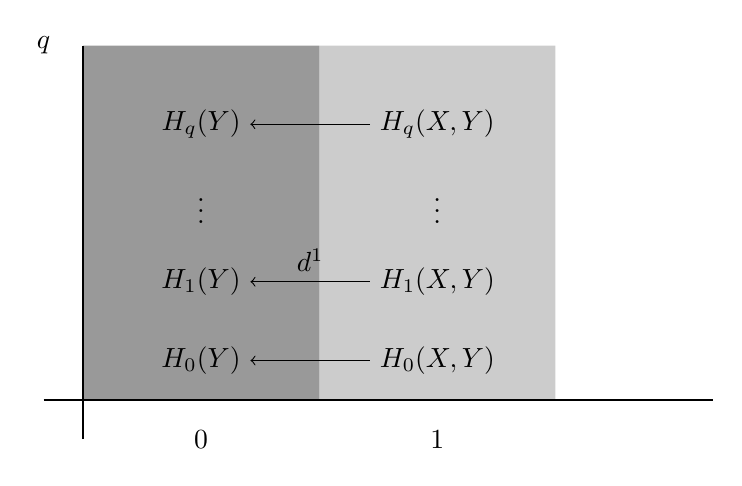
\begin{tikzpicture}
			\fill[opacity=.4] (-1,-0.5) -- (2, -0.5) -- (2,4) -- (-1,4) -- (-1,-0.5);
			\fill[opacity=.2] (2,-0.5) -- (5, -0.5) -- (5,4) -- (2,4) -- (2,-0.5);
			\draw[thick] (-1.5, -0.5) -- (7,-0.5) (-1,-1) -- (-1,4);
			\draw 
			(0.5,3) node(C){$H_{q}(Y)$} (3.5,3) node(D){$H_{q}(X,Y)$}
			(0.5,2) node{$\vdots$}  (3.5,2) node{$\vdots$}
			(0.5,1) node(A){$H_{1}(Y)$} (3.5,1) node(B){$H_{1}(X,Y)$}
			(0.5,0) node(E){$H_{0}(Y)$} (3.5,0) node(F){$H_{0}(X,Y)$};
			\draw (-1.5,4) node{$q$} (0.5,-1) node{$0$} (3.5,-1) node{$1$};
			\draw[->] (B) --node[anchor=south]{$d^{1}$} (A);
			\draw[->] (D) -- (C);
			\draw[->] (F) -- (E);
		\end{tikzpicture}
		\caption{Successione spettrale della coppia $(X,Y)$.}
    	\label{SS-coppia-disegno}
	\end{figure}	
	
	Si può verificare che la mappa di bordo sulla prima pagina
	\begin{equation*}
		d^{1}: E^{1}_{1,q} \longrightarrow E^{1}_{0,q}\,,
	\end{equation*}
	coincide con l'omomorfismo di connessione della coppia
	\begin{equation*}
		\de : H_{q+1}(X,Y) \longrightarrow H_{q}(Y)\,.
	\end{equation*}
	
	Viceversa, supponiamo di avere il dato della successione spettrale
	$(E^{1}_{\bullet, \bullet}, d^{1})$;
	vogliamo ricostruire la successione della coppia.
	Dato che la prima pagina si concentra in due
	colonne adiacenti, è chiaro che la successione 
	collassa alla seconda pagina,
	quindi il termine limite è $E^{\infty}_{\bullet,\bullet} = E^{2}_{\bullet,\bullet}$.
	Per il \hyperref[SS-machine]{Teorema~\ref{SS-machine}},
	calcoliamo il limite per $p=0$ come
	\begin{equation*}
		E^{\infty}_{0,q} = \frac{F_{0}H_{*}}{F_{-1}H_{*}}
		= \frac{\im \left( H_{q}(Y) \to H_{q}(X) \right)}{\im \left( H_{q}(\emptyset) \to H_{q}(X) \right)}
		= \im \left(H_{q}(Y) \xrightarrow{i^{*}} H_{q}(X) \right)\,,
	\end{equation*}
	mentre sulla prima colonna è dato da
	\begin{equation*}
		E^{\infty}_{1,q} = \frac{H_{q+1}(X)}{\im \left( i_{*}: H_{q+1}(Y) \to H_{q+1}(X) \right)}\,.
	\end{equation*}
	D'altra parte la seconda pagina è data da
	\begin{align*}
		E^{2}_{1,q} 
		= \ker \left( H_{q+1}(X,Y) \xrightarrow{\de} H_{q}(Y) \right) \,, \quad
		E^{2}_{0,q} 
		= \frac{H_{q}(Y)}{\im \de} \,.
	\end{align*}
	Confrontando $E^{\infty}$ con la pagina $E^{2}$ si hanno le identità
	\begin{align*}
		E^{2}_{1,q} 
		&= \ker \left( H_{q+1}(X,Y) \xrightarrow{\de} H_{q}(Y) \right) 
		= \frac{H_{q+1}(X)}{\im \left(  H_{q+1}(Y) \to H_{q+1}(X) \right)}
		= E^{\infty}_{1,q}\,, \\
		E^{2}_{0,q} 
		&= \frac{H_{q}(Y)}{\im \de} 
		= \im \left(  H_{q}(Y) \xrightarrow{i^{*}} H_{q}(X) \right)
		= E^{\infty}_{0,q}\,.
	\end{align*}
	dalle quali si ottiene la successione esatta
	\begin{equation*}
		\begin{tikzcd}[column sep=small]
			\cat{0} \ar[r]
			& \frac{H_{q}(Y)}{\im \left(  H_{q+1}(X,Y) \to H_{q}(Y) \right)} \ar[r]
			& H_{q}(X) \ar[r]
			&  \ker \left( H_{q}(X,Y) \xrightarrow{\de} H_{q-1}(Y) \right) \ar[r]
			& \cat{0}\,,
		\end{tikzcd}
	\end{equation*}
	per ogni $q \in \Z$, 
	ovvero la successione della coppia $(X,Y)$.
	Ne segue che la successione della coppia è equivalente alla successione spettrale
	\eqref{SS-coppia}.
\end{ex}




\section{Successioni spettrali di Serre}

Ricordiamo la seguente definizione.

\begin{df}
	Una mappa $\pi : E \to B$ è una \textbf{fibrazione di Serre} se
	vale la \eqref{HLP} sui cubi:
	\begin{equation}\label{Serre-HLP}
		\begin{tikzcd}
			I^{n} \times \{0\} \ar[r] \ar[d, "\iota_{0}"', hook] & E \ar[d, "\pi"] \\
			I^{n+1} \ar[r] \ar[ur, dashed] & B\,. \tag{HLP'}
		\end{tikzcd}
	\end{equation}
\end{df}

Se $B$ è uno spazio connesso per archi che ammette un rivestimento universale $\widetilde{B}$,
allora per il \textbf{Teorema di approssimazione} possiamo trovare un'equivalenza
omotopica debole $f: B' \to B$, con $B'$ un CW complesso. Siccome le fibrazioni
sono una classe chiusa per pullback (vedi \hyperref[fib-prop]{Esercizio~\ref{fib-prop}}), 
allora anche $f^{*}E \to B'$ 
è una fibrazione di Serre, pertanto assumeremo 
senza perdita di generalità che la \emph{base $B$ sia un CW complesso}.

Fissato $x \in B$, consideriamo la fibra $E_{x} = \pi^{-1}(x)$ e
la sua omologia $H_{*}(E_{x})$. 
A ogni cammino
$\gamma : x \mapsto x'$ in $B$ 
vorremmo associare un omomorfismo 
$\gamma_{*} : H_{*}(E_{x}) \to H_{*}(E_{x'})$.
Presa $\alpha_{0} : A_{x} \to E_{x}$ un'approssimazione CW della fibra su $x$,
possiamo usare la \eqref{Serre-HLP} induttivamente sullo scheletro di $A_{x}$
per poter sollevare l'omotopia 
\begin{equation*}
	\Gamma: A_{x} \times I \longrightarrow B\,, \quad
	\Gamma(z,t) := \gamma(t)\,,
\end{equation*}
per ottenere così una mappa diagonale
\begin{equation*}
	\begin{tikzcd}
		A_{x} \times \{0\} \ar[r, "\alpha_{0}"] \ar[d, "\iota_{0}"', hook] & E \ar[d, "\pi"] \\
		A_{x} \times I \ar[r] \ar[ur, dashed, "\alpha"] & B\,. 
	\end{tikzcd}
\end{equation*}
Allora $\alpha_{1} :A_{x} \to E_{x'}$ induce in omotopia un omomorfismo
$\gamma_{*} : H_{*}(E_{x}) \to H_{*}(E_{x'})$.
Notiamo inoltre che se $\gamma \sim \gamma'$ sono omotopi \emph{a estremi fissati},
allora producono lo stesso omomorfismo in omologia; in particolare,
se $x=x'$, notiamo che $\pi_{1}(B,x)$ agisce su
$H_{*}(E_{x})$ e si verifica che se $\gamma$ è costante,
allora induce $\gamma_{*} = \cat{1}_{H_{*}(E_{x})}$.
Questo appena descritto è un esempio di \emph{sistema locale}.

\begin{df}
	Un \textbf{sistema locale di gruppi} $\Gg = \Set{G_{x},\tau_{\gamma}}$ 
	su uno spazio topologico $X$ è un funtore che associa a ogni punto $x \in X$
	un gruppo $G_{x}$ e a ogni cammino $\gamma : I \to X$ da $x_{0}$ a $x_{1}$
	associa un omomorfismo
	\begin{equation*}
		\tau_{\gamma} : G_{x_{0}} \longrightarrow G_{x_{1}}
	\end{equation*}
	che dipende solamente dalla classe
	\begin{equation*}
		[\gamma] \in [(I, \de I) ; (X, \{x_{0}, x_{1} \})]\,,
	\end{equation*}
	con la condizione che se $\gamma$ è costante in $x$, 
	allora l'omomorfismo associato è $\tau_{\gamma} = \cat{1}_{G_{x}}$.
\end{df}

\begin{oss}
	Il gruppo fondamentale $\pi_{1}(B,x)$ agisce (da \emph{sinistra})
	sul gruppo $G_{x}$.
\end{oss}


\begin{oss}
	Siccome ogni cammino $\gamma$ può essere ripercorso in senso
	contrario e produrre il cammino opposto $\overline{\gamma}$
	in modo che la composizione $\gamma \overline{\gamma}$ sia omotopo a una costante,
	deduciamo che ogni $\tau_{\gamma}$ è un isomorfismo.
	In particolare, se $X$ è connesso per archi, allora tutti i $G_{x}$
	di un sistema locale sono isomorfi.
\end{oss}

\begin{df}
	Se l'azione di $\pi_{1}(B,x)$ su $G_{x}$ è banale,
	allora diremo che il sistema locale $\Gg$ è \textbf{banale}.
\end{df}

\begin{ex}
	Ogni sistema locale su uno spazio semplicemente connesso è banale.
\end{ex}


Supponiamo ora che $X$ sia uno spazio connesso per archi
che ammette rivestimento universale $\widetilde{X}$.
Allora $\pi_{1}(X,x_{0})$ agisce (da \emph{destra})
su $\widetilde{X}$ per \textbf{traslazione}, ovvero
\begin{equation*}
	\widetilde{X} \times \pi_{1}(X,x_{0}) \longrightarrow \widetilde{X} \,, \quad
	(x,\gamma) \longmapsto x'\,,
\end{equation*}
dove $x'$ è il punto di arrivo del sollevamento di $\gamma$.
In particolare questo induce un'azione \emph{destra} di $\pi_{1}(X,x_{0})$
sulle catene singolari $C_{*}\left(\widetilde{X}\right)$ per traslazione,
e si verifica che questa azione commuta con il differenziale $d$.

\begin{df}
	Sia $X$ connesso per archi e $\Gg$ un sistema locale su $X$.
	Fissato $x_{0} \in X$, il complesso
	\begin{equation*}
		C_{*}(X;\Gg) := C_{*}\left(\widetilde{X}\right) \otimes_{\Z[\pi_{1}(X,x_{0})]} G_{x_{0}}
	\end{equation*}
	viene chiamato \textbf{complesso delle catene singolari a coefficienti in $\Gg$},
	il cui bordo è indotto da $d:C_{*}(\widetilde{X}) \to C_{*}(\widetilde{X})$.
	Passando al duale, definiamo le \textbf{cocatene singolari a coefficienti in $\Gg$}
	come
	\begin{equation*}
		C^{*}(X;\Gg) := \Hom_{\Z[\pi_{1}(X,x_{0})]}\left(C_{*}\left(\widetilde{X}\right);G_{x_{0}}\right)\,.
	\end{equation*}
	L'\textbf{omologia}, risp. la \textbf{coomologia}, a coefficienti
	in un sistema locale $\Gg$ sarà indicata con
	\begin{equation*}
		H_{*}(X;\Gg) := H_{*}(C_{*}(X;\Gg))\,, \quad
		\text{resp. } H^{*}(X;\Gg) := H^{*}(C^{*}(X;\Gg))\,.
	\end{equation*}
\end{df}


\begin{thm}[\textbf{Successione spettrale di Serre}]\label{Serre-SS}
	Sia $M$ un gruppo abeliano.
	Data una fibrazione di Serre $\pi:E \to B$, con $B$ connesso per archi,
	esiste una successione spettrale $\Set{(E^{r}_{p,q},d^{r})}_{r \ge 2}$
	concentrata nel primo quadrante data da
	\begin{equation*}
		E_{p,q}^{2} = H_{p}\left(B; \Set{H_{q}(E_{x};M)}\right)\,,
	\end{equation*}
	convergente a $E^{\infty}_{p,q} = F_{p}H_{p+q}(E;M)$,
	per una qualche filtrazione $F$ dell'omologia 
	$H_{*}(E;M)$.
\end{thm}

\begin{oss}
	Si noti che nel \hyperref[Serre-SS]{Teorema~\ref{Serre-SS}}
	non vengono nemmeno citati i differenziali della successione spettrale!
\end{oss}

Prima di dimostrare questo risultato,
vediamo alcuni esempi per capirne il funzionamento.

\begin{ex}
	Sia $SU(n)$ il gruppo delle matrici complesse unitarie con determinante $1$.
	Ad esempio, per $n=2$ abbiamo
	\begin{equation*}
		SU(2) = \Set{ \begin{bmatrix} z & \zeta \\ \overline{\zeta} & \overline{z} \end{bmatrix}	
		| {|z|}^{2}	+ {|\zeta|}^{2} = 1 }
		\simeq S^{3}\,.
	\end{equation*}
	La topologia di $SU(3)$ invece è più complicata
	e usiamo il \hyperref[Serre-SS]{Teorema~\ref{Serre-SS}}
	per studiarne l'omologia. La mappa che considera la prima colonna
	\begin{equation*}
		SU(3) \longrightarrow S^{5}\,, \quad
		A \longmapsto A \cdot e_{1}
	\end{equation*}
	dà luogo a una fibrazione $SU(2) \hookrightarrow SU(3) \to S^{5}$.
	La pagina 
	\begin{equation*}
		E_{p,q}^{2} = H_{p}\left(S^{5}; H_{q}(SU(2))\right)
	\end{equation*} 
	della successione spettrale di Serre 
	associata si concentra solo nelle colonne $p=0,5$ e nelle righe $q=0,3$,
	come rappresentato in \hyperref[su3]{Figura~\ref{su3}}. 
	Questo implica che la successione collassa alla seconda pagina,
	e siccome
	$E_{\bullet,\bullet}^{\infty} = E_{\bullet,\bullet}^{2}$,
	si conclude che
		\begin{equation*}
		H_{p}\left( SU(3) \right) =
		\begin{cases}
			\Z\,, \quad &\text{se } p = 0,3,5,8\,;\\
			0\,, \quad &\text{altrimenti.}
		\end{cases}
	\end{equation*}
	
	\begin{figure}
		\centering
		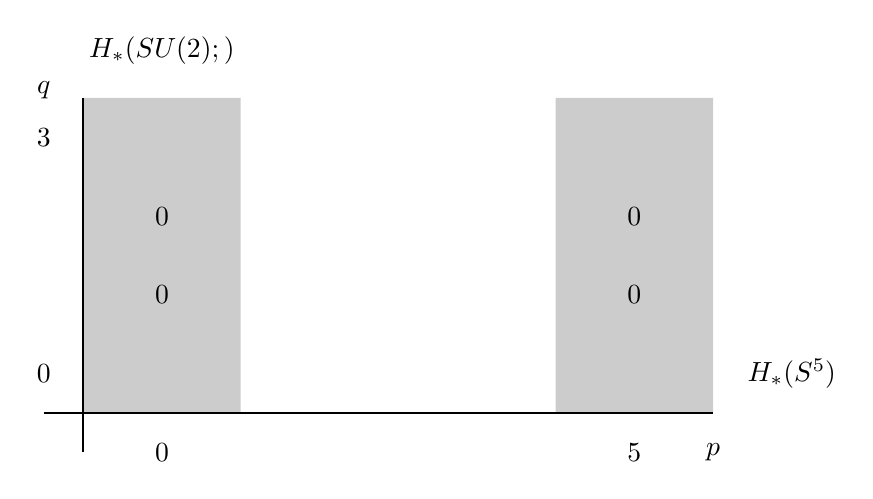
\begin{tikzpicture}
			\fill[opacity=.2] (-1,-0.5) -- (1, -0.5) -- (1,3.5) -- (-1,3.5) -- (-1,-0.5);
			\fill[opacity=.2] (5,-0.5) -- (7, -0.5) -- (7,3.5) -- (5,3.5) -- (5,-0.5);
			\draw[thick] (-1.5, -0.5) -- (7,-0.5) (-1,-1) -- (-1,3.5);
			\draw 
			(0,3) node(A){$\Z$} (6,3) node{$\Z$}
			(0,2) node{$0$}  (6,2) node{$0$}
			(0,1) node{$0$} (6,1) node(B){$0$}
			(0,0) node{$\Z$} (6,0) node{$\Z$};
			\draw 
			(-1.5,3.6) node{$q$} (-1.5,0) node{$0$} (-1.5,3) node{$3$}
			(0,-1) node{$0$} (6,-1) node{$5$} (7,-1) node{$p$};
			\draw (0,4.1) node{$H_{*}(SU(2);\Z)$} (8,0) node{$H_{*}(S^{5})$};
		\end{tikzpicture}
		\caption{Pagina $E^{\bullet,\bullet}_{2}$ della successione di Serre di $SU(3)$.}
    	\label{su3}
	\end{figure}
	
	Possiamo studiare l'omologia
	di $SU(4)$ in maniera analoga: infatti, presa la fibrazione
	\begin{equation*}
		SU(3) \hookrightarrow SU(4) \longrightarrow S^{7}\,,
	\end{equation*}
	otteniamo la successione spettrale la cui pagina $E^{2}_{\bullet,\bullet}$ 
	ha soli $\Z$ concentrati nelle colonne $p=0,7$ e nelle righe $q=0,3,5,8$.
	Si verifica che la successione collassa a questa pagina,
	quindi concludiamo che
	\begin{equation*}
		H_{p}\left( SU(4) \right) =
		\begin{cases}
			\Z\,, \quad &\text{se } p = 0,3,5,7,8,10,12\,;\\
			0\,, \quad &\text{altrimenti.}
		\end{cases}
	\end{equation*}
	
	Infine, vorremmo studiare anche l'omologia di $SU(5)$ 
	utilizzando la fibrazione
	\begin{equation*}
		SU(4) \hookrightarrow SU(5) \longrightarrow S^{9}\,.
	\end{equation*}
	A questo punto $E^{2}_{\bullet,\bullet}$ 
	è come in \hyperref[su5]{Figura~\ref{su5}}
	e notiamo che potrebbero esserci due differenziali non banali.
	Purtroppo non conosciamo la struttura di $d^{9}$,
	quindi (per ora) non sappiamo come calcolare $H_{*}\left( SU(5) \right)$.
	
%		\begin{figure}
%		\centering
%		\begin{tikzpicture}
%			\fill[opacity=.2] (-1,-0.5) -- (1, -0.5) -- (1,3.5) -- (-1,3.5) -- (-1,-0.5);
%			\fill[opacity=.2] (5,-0.5) -- (7, -0.5) -- (7,3.5) -- (5,3.5) -- (5,-0.5);
%			\draw[thick] (-1.5, -0.5) -- (7,-0.5) (-1,-1) -- (-1,3.5);
%			\draw 
%			(0,3) node(A){$\Z$} (6,3) node{$\Z$}
%			(0,2) node{$0$}  (6,2) node{$0$}
%			(0,1) node{$0$} (6,1) node(B){$0$}
%			(0,0) node{$\Z$} (6,0) node{$\Z$};
%			\draw 
%			(-1.5,3.6) node{$q$} (-1.5,0) node{$0$} (-1.5,3) node{$3$}
%			(0,-1) node{$0$} (6,-1) node{$5$} (7,-1) node{$p$};
%			\draw (0,4.1) node{$H_{*}(SU(5);\Z)$} (8,0) node{$H_{*}(S^{9})$};
%		\end{tikzpicture}
%		\caption{Pagina $E^{\bullet,\bullet}_{2}$ della successione di Serre di $SU(3)$.}
%    	\label{su3}
%	\end{figure}
\end{ex}







